\documentclass[border=4pt]{standalone}
\usepackage{tikz}
\usetikzlibrary{arrows.meta,positioning,shapes.geometric}
\begin{document}
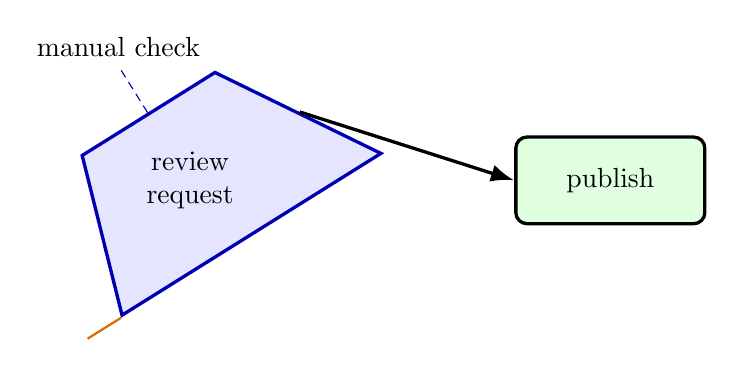
\begin{tikzpicture}[>=Latex,node distance=22mm]
  \node[
    trapezium,
    shape border uses incircle,
    shape border rotate=32,
    trapezium left angle=72,
    trapezium right angle=58,
    minimum width=27mm,
    minimum height=13mm,
    inner sep=1.5mm,
    draw=blue!70!black,
    very thick,
    fill=blue!10,
    align=center
  ] (review) {review\\request};
  \node[draw,very thick,rounded corners,fill=green!12,right=of review,
    minimum width=24mm,minimum height=11mm] (publish) {publish};

  \draw[-Latex,very thick] (review.right side) -- (publish.west);
  \draw[densely dashed,blue!70!black] (review.top side) -- ++(122:7mm)
    node[above,black] {manual check};
  \draw[orange!85!black,thick] (review.bottom left corner) -- ++(212:5mm);
\end{tikzpicture}
\end{document}
